
\documentclass[preprint,12pt]{elsarticle}

\usepackage{graphicx,times,amsmath,amsfonts,subfig,array,multirow,url,algorithm,algorithmic,float,cleveref,pgfplots,bm}
\usepackage[flushleft]{threeparttable}
\usepackage{empheq}
\usepackage{booktabs}
\usepackage{tabularx}
\pgfplotsset{compat=1.12}
\usepackage{xifthen}
\usetikzlibrary{calc, positioning}
\usepackage{color,soul}
\usepackage{tcolorbox}

\journal{Information Sciences}

\begin{document}

\begin{frontmatter}

\title{Multi-Target Support Vector Regression Via Correlation Regressor Chains}

\author[a]{Gabriella Melki}\author[a]{Alberto Cano}\author[a]{Vojislav Kecman}\author[b,c]{Sebasti\'an Ventura}

\address[a]{Department of Computer Science, Virginia Commonwealth University, USA}
\address[b]{Department of Computer Science and Numerical Analysis, University of Cordoba, Spain}
\address[c]{Department of Computer Science, King Abdulaziz University, Saudi Arabia Kingdom}

\begin{abstract}
Multi-target regression is a challenging task that consists of creating predictive models for problems with multiple continuous target outputs. Despite the increasing attention on multi-label classification, there are fewer studies concerning multi-target (MT) regression. The current leading MT models are based on ensembles of regressor chains, where random, differently ordered chains of the target variables are created and used to build separate regression models, using the previous target predictions in the chain. The challenges of building MT models stem from trying to capture and exploit possible correlations among the target variables during training, at the expense of increasing the computational complexity of model training. 
This paper presents three multi-target support vector regression models. The first involves building independent, single-target Support Vector Regression (SVR) models for each output variable. The second builds an ensemble of random chains using the first method as a base model. The third calculates the targets' correlations and forms a maximum correlation chain, which is used to build a single chained support vector regression model. The experimental study evaluates and compares the performance of the three approaches with six other state-of-the-art multi-target regressors. The experimental results are then analyzed using non-parametric statistical tests. The results show that the maximum correlation SVR approach improves the performance of using ensembles of random chains.
\end{abstract}

\begin{keyword}
Multi-target regression \sep multi-output regression \sep regressor chains \sep support vector regressor.
\end{keyword}

\end{frontmatter}

\section{Introduction}
In supervised learning, \textit{single-target} (ST) models are trained to predict the value of a single, categorical or numeric, target attribute of a given example. In some cases, more than one target, or output, can be associated with a single sample input. These situations are handled by a generalization of ST learning, which involves predicting these multiple outputs concurrently, and is known as multi-target (MT) learning~\cite{Aho2012,Borchani2015}. Specifically, MT learning includes \textit{multi-target regression} (MTR), which addresses the prediction of continuous targets, \textit{multi-label classification}~\cite{Zhang20141819} which focuses on binary targets, and \textit{multi-dimensional classification} which describes the prediction of discrete targets~\cite{Borchani2015,Read20141720}. 

Multi-target prediction has the capacity to generate models representing a wide variety of real-world applications, ranging from natural language processing~\cite{Jeong2009} to bioinformatics~\cite{Lui2010}. Other application areas include ecology~\cite{Aho2012}, gene function prediction~\cite{Kocev2015}, predicting the quality of vegetation~\cite{Hadavandi2015-2,Kocev2010}, stock price index forecasting~\cite{Xiong2014}, and operations research~\cite{Borchani2015,Hadavandi2015}. Constructing models for these types of real-world problems presents many challenges, such as missing data, (due to targets not being observed or recorded), and noisy data (due to instrument, experimental or human error), and the curse of high dimensionality. Along with these challenges, the most difficult is identifying patterns between the input data and its corresponding output value. In the context of multi-target modeling, an additional complexity is inherintly created, where multiple outputs must now be trained against. The targets may or may not be correlated, and the corresponding model must accomodate for both scenarios. However, a characteristic of the MT datasets used in these applications and elsewhere, is that they are generated by a single system, most likely indicating that the nature of the outputs captured has some structure~\cite{Hadavandi2015}. Even though modeling the multi-variate nature and possible complex relationships between the target variables is challenging~\cite{Borchani2015}, they are more accurately represented by an MT model.

Several base-line methods have been proposed for solving such multi-target tasks such as Multi-Objective Descision Trees and Random Forests~\cite{Kocev2010}, Boosted Neural Networks~\cite{Hadavandi2015-2}, Ensembles of Trees~\cite{Kocev2013}, and many others. Support Vector Machines are a popular set of linear and non-linear supervised machine learning algorithms with a strong theoretical basis on Vapnik-Chervonenkis theory~\cite{Vapnik1995}. It has previously been shown that they outperform most modeling methods in terms of model performance, scalability, and the ability to efficiently deal with outliers~\cite{Kecman, Drucker1997}. Input space dimensionality does not have an adverse affect on the model training time, and furthermore, the final model produced is sparse, allowing for quick predictions.

There are two main approaches for using such base-line methods in the context of MT learning. The first being \textit{problem transformation} methods, or \textit{local} methods, in which the multi-target problem is transformed into multiple single-target problems, each solved separately using classical methods, as described above. The second being \textit{algorithm adaptation} methods, or \textit{global}, or \textit{big-bang} methods, that adapt existing single-target methods to predict all the target variables simultaneously~\cite{Borchani2015,Kocev2015}.
Using \textit{problem transformation} algorithms for a domain of \textit{t} target variables, \textit{t} predictive models must be constructed, each predicting a single-target variable~\cite{Kocev2015}. Prediction for an unseen sample would be obtained by running each of the \textit{t} single-target models and concatenating their results. Conversely, when using \textit{algorithm adaptation} algorithms for the same domain of \textit{t} target variables, only one model would need to be constructed which would output all \textit{t} predictions.

Literature shows that \textit{algorithm adaptation} methods perform better than \textit{problem transformation} methods~\cite{Kocev2015,Spyromitros2014}. The most valuable advantage of using multi-target techniques is that, not only are the relationships between the sample variables and the targets exploited, but the relationships between the targets amongst themselves are as well~\cite{Baxter1997,Caruana1997}. Single-target techniques, on the other hand, eliminate any possibility of learning from the possible relationships between the target variables because a single, independent model is trained for each target separately~\cite{BenDavic2003}. Another advantage of MT techniques is model interpretability~\cite{Aho2012,Xiong2014}. A single multi-target model is highly more interpretable than a series of single-target models because it not only exploits the relationship between the data and targets, but also the targets amongst themselves. Not only is a single MT model more interpretable, but it could also be considerably more computationally efficient to train, rather than training multiple single-target models individually~\cite{Appice2014}. 

This paper presents three novel approaches to solving multi-target regression problems. The objective of this research topic is to investigate the performance changes when building a regression model using two distinct \textit{algorithm adaptation} chaining methods versus building independent single-target models for each target variable using a novel framework. This paper's contributions includes the following.
\begin{itemize}
\item Using a Support Vector Regressor (SVR) as a \textit{problem transformation} method to determine whether it outperforms current state-of-the-art ST algorithms, while analyzing its performance as a base-line model for MT chaining methods.
\item Building an MT ensemble, using SVR, of randomly chained models (SVRRC), inspired by the classification method, Ensemble of Random Chains Corrected (ERCC)~\cite{Xiong2014}, to investigate the effect of exploiting the possible correlations among target variables.
\item Eliminating the need to test possible correlations of the target attributes using random chains by creating a single chain, built in the direction of maximum correlation among the targets.
\end{itemize}

The experimental study evaluates and compares the performance of the three approaches, together with six other state-of-the-art multi-target regressors, on a set of 19 datasets with varied input size and output targets. The results of the experiments are analyzed using non-parametric statistical analysis, namely the Bonferroni-Dunn and Wilcoxon tests~\cite{Garcia20102044}. These post-hoc tests involve multiple comparisons among the algorithms, where they \st{try and} show significant differences in their performances across all datasets. The statistical analysis of the experiments presented in this paper shows the increase in performance of the support vector regressors, specifically, the maximum correlation chain, SVRCC.

The paper is structured as follows. Section~\ref{sec:background} reviews related works on multi-target regression. Section~\ref{sec:proposal} presents the three multi-target support vector regression approaches. Section~\ref{sec:experiments} presents the experimental study. Section~\ref{sec:results} discusses the results and the statistical analysis. Finally, Section~\ref{sec:conclusions} shows the main conclusions of this work.

\section{Background}\label{sec:background}
This section defines first the notation that will be used in the paper and formally describes the multi-target regression problem along with the relevant state-of-the-art algorithms. 

\begin{table*}[b!]
\renewcommand{\arraystretch}{1.2}
\centering
\caption{Notation}
\begin{threeparttable}
\resizebox{\textwidth}{!}{\begin{tabular}{ll}
\toprule
Definition & Notation\\ 
\midrule
Number of Samples & $\mathcal{N}$ \\
Number of Input Attributes & $d$ \\
Input Space & $\bm{X} = \{\bm X_1, \ldots, \bm X_i, \ldots, \bm X_d\} \in \mathbb{R}^{\mathcal{N} \times d},\,1\leq i \leq d$ \\
Input Instance & $\bm{x}^{(l)} = (x_1^{(l)}, \ldots, x_d^{(l)}) \in \bm{X},\, 1 \leq l \leq\mathcal{N}$ \\
Number of Dataset Targets/Outputs & $m$ \\
Target Space & $\bm{Y} = \{\bm Y_1, \ldots, \bm Y_j, \ldots, \bm Y_m\} \in \mathbb{R}^{\mathcal{N} \times m},\, 1 \leq j \leq m$ \\
\vspace{1.5pt}
Target Instance & $\bm y^{(l)} = (y_1^{(l)}, \ldots, y_m^{(l)}) \in \bm{Y},\,1 \leq l \leq\mathcal{N}$ \\
\hline
\noalign{\vskip 0.04in}
Full Multi-Target (MT) Training Dataset & $\mathcal{D} = \{(x_1^{(1)},y_1^{(1)}), \ldots, (x_d^{(\mathcal N)},y_m^{(\mathcal N)})\}$ \\
Single-Target (ST) Dataset with $j^{th}$ Target & $\mathcal{D}_j = \{(x_1^{(1)},y_j^{(1)}), \ldots, (x_d^{(\mathcal N)},y_j^{(\mathcal N)})\} \in \mathcal{D},\, 1 \leq j \leq m$\\
Number of Cross-Validation (CV) Sets & $k$ \\
ST Test Dataset with $j^{th}$ Target, $i^{th}$ CV Fold & $\mathcal{D}_j^{(i)} = \{(x_1^{(i)},y_j^{(i)}), \ldots, (x_d^{(i)},y_j^{(i)}) \in \mathcal{D}_j,\, i \in \{1,\ldots,\mathcal{N}\}$ \\
ST Training Dataset with $j^{th}$ Target, Excluding the $i^{th}$ CV Fold & $\mathcal{D}_j^{(k-i)} = \mathcal{D}_j \setminus \mathcal{D}_j^{(i)}$ \\
MT Regression Model & $h : \bm{X} \times \bm{Y}$ \\
ST Regression Model & $h_j : \bm{X} \times \bm{Y}_j,\, 1 \leq j \leq m$ \\
Unknown Sample & $\bm{x}^{(\mathcal N^\prime)} = \{\bm {x}^{(\mathcal N+1)}, \ldots, \bm {x}^{\mathcal (N^\prime)}\}$ \\
Predicted Values for Unknown Sample & $\bm{y}^{(\mathcal N^\prime)} = \{\bm{y}^{(\mathcal N+1)}, \ldots, \bm {y}^{(\mathcal N^\prime)}\}$\\
\bottomrule
\end{tabular}}
\end{threeparttable}
\label{tab:Notation}
\bigskip
\end{table*}

\subsection{Notation}\label{subsec:notation}
Let $\mathcal{D}$ be a training dataset of $\mathcal{N}$ instances and their continuous outputs. Let $\bm{X} \in \mathcal{D}$ be a matrix consisting of $d$ input variables and $\mathcal{N}$ samples, sometimes called input space, having a domain of $\bm{X} \in \mathbb{R}^{\mathcal{N} \times d}$. Let $\bm{Y} \in \mathcal{D}$ be a matrix consisting of $m$ target variables for the $\mathcal{N}$ input samples, sometimes called output space, having a domain of $\bm{Y} \in \mathbb{R}^{\mathcal{N} \times m}$. For each sample $(\bm x^{(l)},\bm y^{(l)}) \in \mathcal{D}$, $\bm{x}^{(l)} = (x_1^{(l)}, \ldots, x_d^{(l)})$ and $\bm y^{(l)} = (y_1^{(l)}, \ldots, y_m^{(l)})$ are the input and output vectors respectively, where $l \in \{1, \ldots, \mathcal{N}\}$. Using the training dataset $\mathcal{D} = \{(\bm x^{(1)},\bm y^{(1)}), \ldots, (\bm x^{(\mathcal{N})},\bm y^{(\mathcal{N})})\}$, the goal is to learn a multi-target regression model $h : \bm{X} \times \bm{Y}$, that assigns a vector $\bm{y}$ with $m$ target values, for each input instance $\bm{x}$. The model will then be used to predict the values of $\{\bm{y}^{(\mathcal{N}+1)}, \ldots, \bm{y}^{(\mathcal{N}^\prime)}\}$ for new unlabeled input vectors $\{\bm{x}^{(\mathcal{N}+1)}, \ldots, \bm{x}^{(\mathcal{N}^\prime)}\}$. Table~\ref{tab:Notation} summarizes the notation used in this paper.



\subsection{Multi-Target Regression Methods}\label{subsec:mtr}
In the context of \textit{problem transformation} for multi-target models, $m$ single-target models will be trained on the dataset $\mathcal{D}_j = \{(x_1^{(1)},y_j^{(1)}), \ldots, (x_d^{(N)},y_j^{(\mathcal{N})})\}$, where $j \in \{1, \ldots, m\}$. This way there are $m$ independent, single-target models, one model for each target variable. This is described as the baseline Single-Target (ST) model in~\cite{Spyromitros2014}. A generalized visualization of the \textit{problem transformation} method is shown in Table~\ref{tab:pt}. Many \textit{problem transformation} methods have been proposed to solve multi-target problems, which are detailed next.

\begin{table}[!t]
\renewcommand{\arraystretch}{1.6}
\centering
\caption{Transformation to $m$ Single-Target Datasets}
\begin{tabular}{ccc}
\hline
Dataset & Values & Output \\
\hline
$\mathcal{D}_1$ & $\{(x_1^{(1)},y_1^{(1)}), \ldots, (x_d^{(\mathcal{N})},y_1^{(\mathcal{N})})\}$ & $h_1 : \mathcal{D}_1 \rightarrow \mathbb{R}$ \\
$\mathcal{D}_2$ & $\{(x_1^{(1)},y_2^{(1)}), \ldots, (x_d^{(\mathcal{N})},y_2^{(\mathcal{N})})\}$ & $h_2 : \mathcal{D}_2 \rightarrow \mathbb{R}$ \\
$\vdots$ & $\vdots$ & $\vdots$ \\
$\mathcal{D}_j$ & $\{(x_1^{(1)},y_j^{(1)}), \ldots, (x_d^{(\mathcal{N})},y_j^{(\mathcal{N})})\}$ & $h_j : \mathcal{D}_j \rightarrow \mathbb{R}$ \\
$\vdots$ & $\vdots$ & $\vdots$ \\
$\mathcal{D}_m$ & $\{(x_1^{(1)},y_m^{(1)}), \ldots, (x_d^{(\mathcal{N})},y_m^{(\mathcal{N})})\}$ & $h_m : \mathcal{D}_m \rightarrow \mathbb{R}$ \\
\hline
\end{tabular}
\label{tab:pt}
\end{table}

Multiple authors have proposed Multiple-Target Support Vector Regression methods~\cite{Borchani2015,Xiong2014,Xu2013}. Specifically, \textit{Xiong et. al.} presented a support vector regression method with a firefly heuristic in~\cite{Xiong2014}, in the context of interval forecasting of a stock price index. Originally proposed in~\cite{msvr}, the algorithm was modified in~\cite{Xiong2014} with a firefly heuristic, named FA-MSVR, in order to intelligently identify the appropriate SVR hyper-parameters. Their method for optimizing the FA-MSVR was using an iterative reweighted least squares (IRWLS) approach based on a quasi-Newton strategy. To produce attractive results using support vector machines, appropriate hyper-parameters must be selected. This is a crucial and computationally expensive step to ensure the SVR model is performing to the best of its capabilities~\cite{Zhao2015160}, which is why a firefly heuristic was used in ~\cite{Xiong2014}. The results obtained by \textit{Xiong et. al.} indicate that FA-MSVR proved to be a promising alternate method for time series forecasting, thus highlighting the importance of setting the SVR hyper-parameters. 

Moreover, other approaches based on Linear Target Combinations for MT Regression~\cite{Tsoumakas2014}, and Multi-Objective \st{Decision Trees} \hl{\textbf{Random Forests}}\footnote{This was a typo} (MORF)~\cite{Kocev2007} have been proposed. Most commonly investigated issues for MT learning problems include dimensionality reduction for high-dimensional multi-labeled data. The curse of dimensionality is problematic due to the possible correlations between the data and the targets~\cite{Charte20141842,Ding20152521,He2011}. This multi-collinearity may cause the learning task to be more difficult and complex~\cite{Qian2015594}. To reduce the dimensionality of the data, without losing the possible relationships to the targets, careful feature selection could be performed, which is a difficult task as well~\cite{Lee201580,Li2016827}. Another issue would be processing large datasets quickly and feasibly (because of memory constraints), while providing insightful information~\cite{Borchani2015, 2016-INS-LAIM}.

The MTS, MTSC, ERC, and ERCC methods are introduced by \textit{Spyromitros et. al.} in~\cite{Spyromitros2014}. The idea behind these algorithms was to investigate whether advances in multi-label learning can be successfully used and implemented in a multi-target regression setting, as well as shedding light on modeling target dependencies. They first describe the MTS and ERC models, which are both inspired by multi-label classification algorithms, and then introduce their corrected versions. These two methods involve two stages of learning, the first being building ST models and the second uses the knowledge gained by the first step to predict the target variables while using possible relationships the target variables might have with one another. 

The two stages of training in MTS involve firstly, training $m$ independent single-target models, like in ST. In the second step, a second set of $m$ meta models are learned for each target variable, $\bm{Y}_j,\, 1 \leq j \leq m$. These meta models are learned on a transformed dataset, where the input attributes space is expanded by adding the approximated target variables obtained in the first stage, excluding the $j^{th}$ target being predicted. Each $m$ meta model, $h_j^* : \bm{X} \times \mathbb{R}^{m-1} \rightarrow \mathbb{R}$, is learned by the modified dataset $\mathcal{D}_j^* = \{(x_1^{*(1)},y_j^{*(1)}), \ldots, (x_d^{*(\mathcal{N})},y_j^{*(\mathcal{N})})\}$, where $\bm x_j^{*(l)} = \{x_1^{(l)}, \ldots, x_d^{(l)}, \hat{y}_1^{(l)}, \ldots, \hat{y}_{j-1}^{(l)}, \hat{y}_{j+1}^{(l)}, \ldots, \hat{y}_m^{(l)}\},\, l \in \{1, \ldots, \mathcal{N}\}$ are the input vectors along with the $m-1$ predicted target variables, represented by $\hat{\bm y}$, obtained by the first step. To predict the output for a new input vector $\bm{x}^{(q)}$, the models trained in the first stage are applied and an output vector, $\hat{\bm{y}}^{(q)} = \{\hat{\bm{y}}_1^{(q)}, \ldots, \hat{\bm{y}}_m^{(q)}\} = \{h_1(\bm{x}^{(q)}), \ldots, h_m(\bm{x}^{(q)})\}$, is obtained. The second stage models are then applied on the transformed input vector $\bm x_j^{*(q)}$, as shown above, to produce a final output vector.

%\subsubsection{Ensembles of Random Chains}

The ERC method is somewhat similar to the MTS method. In the training of a Regression Chain (RC) model, a random chain, or sequence, of the set of target variables is selected and for each target in the chain, models are built sequentially by using the output of the previous model as input for the next~\cite{Xioufis2016}. If the default, ordered chain is $C = \{\bm Y_1, \bm Y_2, \ldots, \bm Y_m\}$, the first model $h_1 : \bm X \rightarrow \mathbb{R}$ is trained for $\bm Y_1$, as in ST. For the subsequent models $h_{j,j>1}$, the dataset is transformed into $\mathcal{D}_j^* = \{(\bm x_j^{*(1)},y_j^{(1)}), \ldots, (\bm x_j^{*(\mathcal{N})},y_j^{(\mathcal{N})})\}$, where $\bm x_j^{*(l)} = \{x_1^{(l)}, \ldots, x_d^{(l)}, y_1^{(l)}, \ldots, y_{j-1}^{(l)}\}$ are the input vectors transformed by sequentially appending the true values of each of the previous targets in the chain. For a new input vector $\bm{x}^{(q)}$, the target values are unknown. So  once the models are trained, the unseen input vector $\bm{x}^{(q)}$ will be appended with the approximated target values, making the models dependent on the approximated values obtained in each step. One of the issues associated with this method is that, if a single random chain is used, the possible relationships between the targets at the head of the chain and the end of the chain are not exploited due to the algorithm's sequential nature. Also, prediction error in the earlier stages of the models will be propagated as the rest of the models are trained, which is why the Ensemble of Regressor Chains was proposed in ~\cite{Spyromitros2014}. Instead of a single chain, $k$ chains are created at random, and the final prediction values are obtained by taking the mean values of the $k$ predicted values for each target. 

In the methods described above, the estimated target variables (meta-variables) are used as input in the second stage of training. In both methods, the models are trained using these meta-variables that become noisy at prediction time, and thus the relationship between the meta-variables and target variable is muddied. Dividing the training set into sets, one for each stage, would not help this situation because both methods would be trained on training sets of decreasing size. Due to these issues, \textit{Spyromitros et. al.} proposed modifications, in \cite{Spyromitros2014}, to both methods that resembles $k$-fold cross-validation (CV) to be able to obtain unbiased estimates of the meta-variables. These methods are called Regression Chains Corrected (RCC) and Multi-Target Stacking Corrected (MTSC). 

The ERCC and MTSC procedures involve repeating the RCC and MTS procedures $k$ times, respectively, with $k$ randomly ordered chains for ERCC, and $k$ different modified training sets for MTSC. The algorithms were tested and compared using Bagging of $100$ regression trees as their base regression algorithm with ERC and ERCC ensemble size of $10$, and $10$-fold cross-validation. The corrected methods exhibited better performance than their original variants, as well as ST models. The ERCC algorithm had the best overall performance, as well as being statistically significantly more accurate of all the methods tested. These methods can be found and used through the open-source Java library, Mulan~\cite{mulan}; to replicate the results found in~\cite{Spyromitros2014}. 

The following section presents our approaches to solving the multi-target regression problem inspired by the techniques presented in~\cite{Spyromitros2014}. It will show that exploiting and making use of the possible correlations in the target variables produces better results than not. 

\section{Multi-target SVR proposal}\label{sec:proposal}

Three novel models have been implemented for the purposes of multi-target regression. The \st{base model} \hl{\textbf{base-line model}} is the SVR model, where $m$ single-target soft-margin non-linear support vector regressors (NL-SVR) are built for each target variable $\bm Y_j$. For NL-SVR, the regularized soft-margin loss function given in equation \eqref{eq:softsvropt} is minimized~\cite{Drucker1997,Kecman},

\begin{subequations}\label{eq:softsvropt}
\begin{equation}
\begin{aligned}
\underset{\bm{w},\xi,\xi^*}{\text{minimize}} & \ \ \ \ \frac{1}{2}||\bm{w}||^2 + C\sum_{l=1}^\mathcal{N}{\left(\xi^{(l)} + \xi^{*(l)} \right)}
\end{aligned}
\tag{\ref{eq:softsvropt}}
\end{equation}
\begin{empheq}[left={\text{subject to}\  }\empheqlbrace]{align}
y^{(l)}-\langle \bm{w},\phi\left(\bm{x}^{(l)}\right)\rangle \leq \epsilon + \xi^{(l)} \\
\langle \bm{w},\phi\left(\bm{x}^{(l)}\right)\rangle-y^{(l)} \leq \epsilon + \xi^{*(l)} \\
\xi^{(l)}, \xi^{*(l)} \geq 0 
\end{empheq}
\end{subequations}

where $\bm{w}$ represents the SVR weight vector, $\epsilon$ represents how precise the approximations are, $C > 0$ determines how to penalize deviations from $\epsilon$, $\phi(\cdot)$ represents a feature mapping function, $\xi^{(l)}$ and $\xi^{*(l)}$ are slack variables, and $y^{(l)}$ is the label corresponding to the input vector $\bm{x}^{(l)}$. For simplicity, the bias SVR term has been excluded. In our algorithm implementation, the dual of this formulation~\cite{Vapnik1995,Drucker1997} given by \eqref{eq:dualsvr} is solved,

\begin{subequations}\label{eq:dualsvr}
\begin{equation}
\begin{aligned}
\underset{\bm{\alpha},\bm{\alpha}^*}{\text{maximize}} & \ \ \ -\frac{1}{2}\sum_{l,k=1}^{\mathcal{N}}{\left(\bm{\alpha}^{(l)}-\bm{\alpha}^{*(l)}\right)\left(\bm{\alpha}^{(k)}-\bm{\alpha}^{*(k)}\right)}\mathcal{K}\left(\bm{x}^{(l)},\bm{x}^{(k)}\right)\\
{} & -\epsilon\sum_{l=1}^{\mathcal{N}}{\left(\bm{\alpha}^{(l)}+\bm{\alpha}^{*(l)}\right)} + \sum_{l=1}^{\mathcal{N}}{y^{(l)}\left(\bm{\alpha}^{(l)}-\bm{\alpha}^{*(l)}\right)} 
\end{aligned}
\tag{\ref{eq:dualsvr}}
\end{equation}
\begin{eqnarray}
\text{subject to} & \sum_{l=1}^{\mathcal{N}}{\left(\bm{\alpha}^{(l)}-\bm{\alpha}^{*(l)}\right)=0},\ \ \bm{\alpha}^{(l)},\bm{\alpha}^{*(l)} \in \left[0,C\right]
\end{eqnarray}
\end{subequations}

where the $\boldsymbol{\alpha}$ and $\boldsymbol{\alpha^*}$ vectors correspond to the SVR dual variables and \\$\mathcal{K}\left(\bm{x}^{(l)},\bm{x}^{(k)}\right) = \phi(\bm{x}^{(l)})^\prime * \phi(\bm{x}^{(k)})$ is an $\left({\mathcal{N}} \times {\mathcal{N}}\right)$ Gaussian kernel matrix which is dependent on the $\gamma$ parameter for its broadness. Using the SVR optimization problem described, the multi-target problem is solved by transforming it into $m$ single-target problems, as shown in Algorithm~\ref{alg:SVR}. This algorithm will output $m$ single-target models, $h_j,\,\forall j = 1,\ldots,m$, for a given dataset $\mathcal{D}$. It first splits the dataset into $m$ separate ones, each with a single-target variable $\bm Y_j$, and then builds a distinct SVR model for each of the datasets. 

\begin{algorithm}[t!]
\caption{MT Support Vector Regression (SVR)}
\label{alg:SVR} 
\begin{algorithmic}[1]
\renewcommand{\algorithmicrequire}{\textbf{Input:}}
\renewcommand{\algorithmicensure}{\textbf{Output:}}
\REQUIRE Training dataset $\mathcal{D}$, number of cross-validation folds $k$
\ENSURE  ST models $h_j, j = 1,\ldots,m$
\\ \textit{Build $m$ ST SVR Models}
\FOR {$j = 1$ to $m$}
\STATE $\mathcal{D}_j = \{(x_1^{(1)},y_j^{(1)}), \ldots, (x_d^{(\mathcal N)},y_j^{(\mathcal N)})\}$
\\ \textit{Create the CV training $\mathcal{D}^{(k-i)}$ and test $\mathcal{D}^{(i)}$ sets}
\FOR {$i=1$ to $k$}
\STATE $\mathcal{D}_j^{(k-i)} = \{(x_1^{(k-i)},y_j^{(k-i)}), \ldots, (x_d^{(k-i)},y_j^{(k-i)})\}$ 
\STATE $\mathcal{D}_j^{(i)} = \{(x_1^{(i)},y_j^{(i)}), \ldots, (x_d^{(i)},y_j^{(i)})\}$ 
\\ \textit{Train the $j^{th}$ model on the training set $\mathcal{D}^{(k-i)}$}
\STATE $h_j^{(k-i)} : \mathcal{D}_j^{(k-i)} \rightarrow \mathbb{R}$
\\ \textit{Test the $j^{th}$ model on the test set $\mathcal{D}^{(i)}$}
\STATE $\hat{\bm Y}_j^{(i)} = h_j^{(k-i)}(\bm X^{(i)})$
\ENDFOR
\\ \textit{Calculate and store aRRMSE error for the $j^{th}$ model}
\ENDFOR
\RETURN $h_j, j=1,\ldots,m$ 
\end{algorithmic} 
\end{algorithm}

Building $m$ ST models was a good base-line model, but as mentioned previously, it does not use any of the possible correlations between the target attributes during training. If these correlations are not exploited, it could retract from the model's potential performance. Therefore, we also proposed to construct a series of random chains and create an ensemble model, as done in~\cite{Spyromitros2014}, but using our base-line SVR method, named SVR Random Chains (SVRRC). For SVRRC, ensembles of at most $10$ random chains are built, with length $m$, of different and distinct permutations of the target variable indices. For each chain, we train $m$ chained models using the targets true values. Due to the computational complexity of building $m!$ distinct chains and training $\left(m!\right) \times m$ models, the number of ensembles and chains are limited to a maximum of $10$, as proposed by \textit{Spyromitros et. al.} in~\cite{Spyromitros2014}. However, if the number of target variables is less than $3$, i.e. $m! \leq 10$, we construct all $m!$ random chains.

For each of the random chains, the model is trained by predicting the first target variable in the chain. Next, the first target's true value, $\bm Y_j$, is appended to the end of the training set as such, $\mathcal{D}_{j+1}^* = \{\bm X_{j+1}^*, \bm Y_j\}$, where $\bm X_{j+1}^*$ is the appended training set, ${\bm X_{j+1}^* = \{x_1^{(l)},\ldots,x_d^{(l)},y_1^{(l)},\ldots,y_j^{(l)}\},l=\{1,\ldots,\mathcal N\}}$. 

The chaining process is repeated for all the target indices in the chains. When chaining target values, there are two main options: using the predicted value as input for the following target, or using the true value of the target variable as input of the subsequent targets. The main problem with the former approach is that errors are propagated, while the latter minimizes error propagation and results in better accuracy results. Our approach and the other methods compared employ chaining of the true values. Given the ensemble of SVRs, the predicted values for a given instance are calculated by taking the mean of the multiple models generated using different random chains. For predicting unseen inputs that have no target values, the predicted value at each step of the chain $\hat{y_j}^{(l)}$ is appended to the input as shown in Algorithm~\ref{alg:SVRCP}. For SVRRC described in Algorithm~\ref{alg:SVRRC}, at most $10$ models will be built (one for each chain $RC$, $RC_c = \{RC_c^{(1)}, \ldots, RC_c^{(m)}\}, \, c \leq 10 \,$), each iterating and training $m$ chained models. For each of the models in the chain, we use $10$-fold cross-validation to ensure the hyper-parameters chosen best describe the data. 

\begin{algorithm}[t!]
\caption{MT SVR with Random-Chains (SVRRC)}
\label{alg:SVRRC} 
\begin{algorithmic}[1]
\renewcommand{\algorithmicrequire}{\textbf{Input:}}
\renewcommand{\algorithmicensure}{\textbf{Output:}}
\REQUIRE Training dataset $\mathcal{D}$, number of cross-validation folds $k$
\ENSURE  $c$ chained models $h_j, j = \{1,\ldots,m\}, c \leq 10$
\\ \textit{Create at most $10$ distinct random chains of size $m$}
\STATE $RC_c^{(m)}$
\\ \textit{Create ST transformation of $\mathcal{D}$ with the $1^{st}$ index in chain $c$}
\STATE $\mathcal{D}_1^* = \{(x_1^{(1)},y_1^{(1)}),\ldots,(x_d^{(\mathcal N)},y_1^{(\mathcal N)})\}$
\\ \textit{Build $m$ chained models for each chain $c \in \{1,\ldots,10\}$}
\FOR {$j=1$ to $m$}
\STATE $h_j : \mathcal{D}_j^* \rightarrow \mathbb{R}$
\\ \textit{Initialize appended dataset, $\mathcal{D}_{j+1}^*$}
\IF {$j < m$}
\STATE $\mathcal{D}_{j+1}^* \leftarrow \emptyset$
\\ \textit{Split $\mathcal{D}_j^*$ into $k$ disjoint parts $\mathcal{D}_j^{*(i)}, \, i=1,\ldots,k$ for training and testing}
\FOR {$i=1$ to $k$}
\STATE $h_j^{(i)} : \mathcal{D}_j^{(k-i)} \rightarrow \mathbb{R}$
\\ \textit{Test the model on the test set $D_j^{*(i)}$}
\FOR {$\bm x^{*(i)} \in \mathcal{D}_j^{*(i)}$}
\STATE $\hat{y}_j^{(i)} = h_j^{(i)}(\bm x^{*(i)})$
\\ \textit{Append $\bm x^{*(i)}$ with the true value $y_j^{(i)}$, and add it to set $\mathcal{D}_{j+1}^*$}
\STATE $\mathcal{D}_{j+1}^* = \mathcal{D}_{j+1}^* \cup [\bm x^{*(i)},y_j^{(i)}]$
\ENDFOR
\ENDFOR
\ENDIF
\ENDFOR
\RETURN $h_j, j=1,\ldots,m$ 
\end{algorithmic} 
\end{algorithm}

\begin{algorithm}[t!]
\caption{SVR Chained Prediction}
\label{alg:SVRCP} 
\begin{algorithmic}[1]
\renewcommand{\algorithmicrequire}{\textbf{Input:}}
\renewcommand{\algorithmicensure}{\textbf{Output:}}
\REQUIRE Unknown sample $\bm x^{(q)}$, chained model ${h_j, j=\{1...m\}}$
\ENSURE  Output vector $\hat{\bm y}^{(q)}$ of size $m$
\\ \textit{Initialize the output vector}
\STATE $\hat{\bm y}^{(q)} = \textbf{0}$
\\ \textit{Initialize the input space for the first target}
\STATE $\mathcal{D}_1^* = \bm x^{(q)}$
\FOR {$j=1$ to $m$}
\STATE $\bm x^* \in \mathcal{D}_j^*$
\STATE $\hat{y}_j^{(q)} = h_j(\bm x^*)$
\STATE $\mathcal{D}_{j+1}^* = \mathcal{D}_j^* \cup [\bm x^*, \hat{y}_j^{(q)}]$
\ENDFOR
\\ \textit{Create ST transformation of $\mathcal{D}$ with $1^{st}$ index in chain $c$}
\RETURN $\hat{\bm y}^{(q)}$ 
\end{algorithmic} 
\end{algorithm}

\begin{algorithm}[t!]
\caption{MT SVR with Max-Correlation Chain (SVRCC)}
\label{alg:SVRCC} 
\begin{algorithmic}[1]
\renewcommand{\algorithmicrequire}{\textbf{Input:}}
\renewcommand{\algorithmicensure}{\textbf{Output:}}
\REQUIRE Training dataset $\mathcal{D}$, number of cross-validation folds $k$
\ENSURE  Chained model $h_j, j = \{1,\ldots,m\}$
\\ \textit{Find maximum correlation chain for the target variables}
\STATE $correlation_{\left(m \times m\right)} = corrcoef(\bm Y)$
\STATE $sums_m = sum\left(correlation\left(l,j\right)\right), l=1,\ldots,m$
\\ \textit{Create the maximum correlation chain $c$ of size $m$}
\STATE $c_m = sort\left(sums_m,\textbf{decreasing}\right)$
\STATE $\mathcal{D}_{c_1}^* = \{(x_1^{(1)},y_{c_1}^{(1)}),\ldots,(x_d^{(\mathcal N)},y_{c_1}^{(\mathcal N)})\}$
\\ \textit{Build a chained model, for max-chain $c_m$}
\FOR {$j=1$ to $m$}
\STATE $h_{c_j} : \mathcal{D}_{c_j}^* \rightarrow \mathbb{R}$
\\ \textit{Initialize appended dataset, $\mathcal{D}_{c_{(j+1)}}^*$}
\IF {$j < m$}
\STATE $\mathcal{D}_{c_{j+1}}^* \leftarrow \emptyset$
\\ \textit{Split $\mathcal{D}_{c_j}^*$ into $k$ disjoint parts $\mathcal{D}_{c_j}^{*(i)}, \, i=1,\ldots,k$ for training and testing}
\FOR {$i=1$ to $k$}
\STATE $h_{c_j}^{(i)} : \mathcal{D}_{c_j}^{*(k-i)} \rightarrow \mathbb{R}$
\\ \textit{Test the model on the test set $\mathcal{D}_{c_j}^{*(i)}$}
\FOR {$\bm x^{*(i)} \in \mathcal{D}_{c_j}^{*(i)}$}
\STATE $\hat{y}_{c_j}^i = h_{c_j}^{(i)}(\bm x^{*(i)})$
\\ \textit{Append $\bm x^{*(i)}$ with the true value $y_{c_j}^{(i)}$, and add it to set $\mathcal{D}_{c_{(j+1)}}^*$}
\STATE $\mathcal{D}_{c_{(j+1)}}^* = \mathcal{D}_{c_{(j+1)}}^* \cup [\bm x^{*(i)},y_{c_j}^{(i)}]$
\ENDFOR
\ENDFOR
\ENDIF
\ENDFOR
\RETURN $h_j, j = \{1,\ldots,m\}$
\end{algorithmic} 
\end{algorithm}

When the number of output variables increases, the number of possible chains increases factorially. Therefore, there is no guarantee that the random chains generated will truly reflect the relationships among the target variables. Moreover, building an ensemble of regressors is computationally expensive. Finding a heuristic that allows the identification of a single, most appropriate chain, which fully reflects the output variable interrelations would improve the computational complexity of training the ensemble. Our third proposal builds a single chain based on the maximization of the correlations among the target variables. By calculating the correlation of the target variables and imposing that on the order of the chain, we ensure that each appended target provides some additional knowledge on the training of the next. With SVRRC, there is no proof or reasoning behind the generation of these chains, and since the number of random chains generated is limited to $10$, there is no way of ensuring that the $10$ chains fully represent the targets' dependencies. Therefore, calculating and using the correlations of the targets would break this uncertainty, as done in Algorithm~\ref{alg:SVRCC}, the SVR Correlation Chain (SVRCC) method. The computational complexity and hardware constraints (memory size) are negligible during the construction of the targets' correlation matrix, since the correlation matrix would be an $(m \times m)$ matrix, and the likelihood that the number of targets is large enough to cause a memory issue is minimal. To calculate the correlation coefficients of the targets, we first construct the targets' co-variance matrix, $\sum_{i,j} = cov(Y_i,Y_j) = \mathbf{E}\left[(Y_i - \mu_i)(Y_j - \mu_j)\right]$, where $\mu_i = \mathbf{E}(Y_i)$, and $\mathbf{E}(Y_i)$ is the expected value of $Y_i$, $\forall i,j \in \{1,\ldots,m\}$. This matrix will show how the targets change together. We then calculate the correlation coefficients matrix $\rho_Y = corrcoef(Y) = \frac{cov(Y_i,Y_j)}{\sqrt{cov(Y_i,Y_i)cov(Y_j,Y_j)}}$, $\forall i,j \in \{1,\ldots,m\}$. The correlation coefficients matrix will describe the linear relationship among the target variables and we can then sort them in decreasing order, creating our maximum correlation chain. Having a single chain reduces the computational complexity, while providing a competitive model. For an unknown sample, the prediction method is the same as Algorithm~\ref{alg:SVRCP}. 



\section{Experiments}\label{sec:experiments}
This section presents the experimental comparison of the three models proposed, along with six others from state-of-the-art. It introduces the datasets, algorithms, and performance measures. 

\subsection{Datasets}\label{subsec:data}
This section presents a description of the datasets used in the experiments. Although there are many interesting applications of multi-target regression, there are not many publicly available datasets to use. The datasets used in the experimental study were collected from the Mulan website~\cite{mulan}, as well as the UCI Machine Learning Repository~\cite{Lichman:2013}. Information on the $19$ datasets used is summarized in Table~\ref{tab:datasets}, where the number of samples, attributes (dimensionality), and targets are shown. Note that the datasets used in this experiment are the same datasets used in~\cite{Spyromitros2014} to properly perform our model comparisons, as well as some additional datasets. 

\begin{itemize}
\item \textbf{Electrical Discharge Machining} The EDM dataset's purpose is to optimize the machining time by approximating the behavior of a human operator who controls the values of two variables, gap control and flow control. 
\item \textbf{Solar Flare 1 \& Solar Flare 2} The Solar Flare dataset~\cite{mulan} is used for predicting how often 3 types of solar flare are observed in 24 hours. The three types of solar flare - common, moderate, and severe. 
\item \textbf{Water Quality} The Water Quality dataset~\cite{mulan} is used for approximating 14 target attributes that represent chemicals found in Slovenian rivers. 16 input attributes describing the biology of the river, the chemistry and physical water quality, are used to predict the target variables.
\item \textbf{OES97 \& OES10} The Occupational Employment Survey datasets~\cite{mulan} were compiled during the years 1997 (OES97) and 2010 (OES10). There are 16 targets that are randomly selected from a set of employment categories.
\item \textbf{ATP1d \& ATP7d} The Airline Ticket Price datasets~\cite{mulan} are used to predict airline ticket prices. The 411 input variables include details about the different flights and the 6 targets are the minimum prices observed over the next 7 days for 6 airline preferences. 
\item \textbf{SCM1d} The Supply Chain Management dataset~\cite{mulan} is used to predict how likely a product is to succeed. The input variables are the observed prices for a specific day, and 4 projected prices. Each of the 16 target variables correspond to the next day mean price for each of the products. 
\item \textbf{Wisconsin Cancer} Each sample represents follow-up data for one breast cancer patient, who is exhibiting invasive breast cancer, and no evidence of metastases at the time of diagnosis. This dataset can be used to predict whether the cancer is recurrent, and the time in which it might recur. 
\item \textbf{Stock} This dataset includes the daily stock prices from January $1988$ through October $1991$ for $10$ aerospace companies.
\item \textbf{California Housing} This dataset includes information on block groups of individuals in California, from the $1990$ Census. It contains $20,640$ samples with $7$ continuous attributes, which are used to predict the $2$ target variables, median house value and the median income.
\item \textbf{Puma8NH \& Puma32H} The Puma8H and Puma32H datasets are synthetically generated from a simulation of the dynamics of a Unimation Puma 560 robot arm~\cite{Lichman:2013}, used to predict the angular acceleration of one robot arm link. The inputs, 8 for Puma8H and 32 for Puma32H, include angular positions, velocities, and torques of the robot arm.
\item \textbf{Friedman} This is an artificial dataset where $25$ attributes of each of the samples are generated independently from a uniform distribution over $[0,1]$. To measure the effects of non-related attributes, additional attributes are added to the datasets, which are independent from the output. 
\item \textbf{Polymer} The Polymer Test Plant dataset contains $10$ input variables representing measurements of controlled variables, such as temperatures, feed rates, etc, in a polymer processing plant. The $4$ target variables are the measurements of the output of that plant.
\item \textbf{M5SPEC \& MP5SPEC \& MP6SPEC} These datasets consist of $80$ samples of corn measured on $3$ different NIR spectrometers, M5, MP5, and MP6.
\end{itemize}

\begin{table*}[!t]
\renewcommand{\arraystretch}{1.2}
\centering
\caption{Multi-Target Regression datasets}
\begin{tabular}{lccc}
\hline
Dataset & Samples $(\mathcal N)$ & Attributes $(d)$ & Targets $(m)$\\
\hline
EDM & 145 & 16 & 2\\
Solar Flare 1 & 323 & 10 & 3\\
Solar Flare 2 & 1,066 & 10 & 3\\
Water Quality & 1,060 & 16 & 14\\
OES97 & 323 & 263 & 16\\
OES10 & 403 & 298 & 16\\
ATP1d & 201 & 411 & 6\\
ATP7d & 188 & 411 & 6\\
SCM1d & 9,125 & 280 & 16\\
Wisconsin Cancer & 198 & 34 & 2\\
Stock & 950 & 10 & 3\\
California Housing & 20,640 & 7 & 2\\
Puma8NH & 8,192 & 8 & 3\\
Puma32H & 8,192 & 32 & 6\\
Friedman & 500 & 25 & 6\\
Polymer & 41 & 10 & 4\\
M5SPEC & 80 & 700 & 3\\
MP5SPEC & 80 & 700 & 3\\
MP6SPEC & 80 & 700 & 3\\
\hline
\end{tabular}
\label{tab:datasets}
\end{table*}

\subsection{Algorithms}\label{subsec:algorithmsres}
This section presents the algorithms that we compare our proposals' performances to; namely ST, MTS, MTSC, ERC, ERCC, and MORF which has been used in the experimental study conducted in~\cite{Spyromitros2014}. Our contributions are compared to these algorithms because they have shown considerable performance in training multi-target models. The have also made their framework readily available for reproducing their results, allowing proper comparisons to be made with their methods. Moreover, note that all three SVR algorithms are implemented within the general framework of Mulan's MTRegressor\footnote{http://mulan.sourceforge.net}~\cite{mulan}, which was built on top of Weka\footnote{http://www.cs.waikato.ac.nz/ml/weka}~\cite{weka}, and we also used LIBSVM's Epsilon-SVR~\cite{CC01a} implementation of Support Vector Regressors as the base SVR model.

In order to train a model that accurately describes a dataset and is not over-fit, one must experiment with different model hyper-parameters. In the case of SVMs and the SVM regression task, these parameters are the penalty parameter $C$, the Gaussian kernel parameter $\gamma$, and the error or tube parameter $\epsilon$. We experimented with a range of parameters given in equations~\eqref{eq:paramC} to~\eqref{eq:paramE}, referred to as~\eqref{eq:hyperparam}, to ensure the final model is best representative of the dataset the model is being trained on.
\begin{subequations}
\label{eq:hyperparam}
\begin{align}
C \in  & \{1, 10, 100\} \label{eq:paramC}\\
\gamma \in  & \{1^{-9}, 1^{-7}, 1^{-5}, 1^{-3}, 1^{-1}, 1, 5, 10\} \label{eq:paramG}\\
\epsilon \in  & \{0.01, 0.1, 0.2\} \label{eq:paramE}
\end{align}
\end{subequations}

%SVR Parameter selection using internal 10-fold cross validation
We have compared the models trained on the different hyper-parameters using the cross-validation procedure which ensures that the models' performances are accurately assessed and the model built is not biased towards the full dataset. %For each cross-validation loop, the data is separated into equally sized sections; in our experiments we have chosen to use $10$ folds. Each part is held out in turn as the test set, and the remaining nine parts are used as the training set. By doing this we are ensuring the model built is not biased towards the full dataset. 

To ensure having a controlled environment when conducting our performance comparisons, the experimental environment for running the competing algorithms was the same as what was done in~\cite{Spyromitros2014}. This includes the following. The ST base-line model used was Bagging~\cite{Breiman1996} of 100 regression trees~\cite{Wu2015430}. The MTSC and ERCC methods are run using $10$-fold cross-validation, and the ensemble size for the ERC and ERCC methods was set to $10$. The ensemble size of 100 trees was used for MORF, and the rest of its parameters were set as recommended by~\cite{Kocev2013}.

The main preprocessing step used for the experiments was normalization. The input variables were scaled to have a mean value of $0$ and standard deviation of $1$. To ensure that each sample is definitely used when building the final model, we used sampling without replacement when creating our training and testing sets.
The preprocessed and final datasets used in the experiments, along with the code for the algorithms presented in this paper, can be publicly found here:\\ ~\url{http://people.vcu.edu/~acano/MTR-SVRCC}

\subsection{Performance Evaluation}\label{subsec:perfeval}
The performance metric used to analyze our contributions' performances is shown in Equation~\ref{eqn:aarmse}. For unseen or test datasets of size $\mathcal N_{test}$, the performances are evaluated by taking the average, relative root mean square error (aRRMSE)~\cite{Borchani2015,Friedman2010} given by,
\begin{eqnarray}{c}
\textit{aRRMSE} = \frac{1}{m} \sum_{j = 1}^m \sqrt{\frac{\sum_{l = 1}^{\mathcal N_{test}} (y_j^{(l)} - \hat{y}_j^{(l)})^2}{\sum_{l = 1}^{\mathcal N_{test}} (y_j^{(l)} - \bar{y}_j)^2}}
\label{eqn:aarmse}
\end{eqnarray}
where $\hat{\textbf{y}}$ is the predicted output and $\bar{\textbf{y}}$ is the average of the true output target variable. The test dataset is the hold-out set during cross validation. This ensures our model is evaluated on data that it has not been trained on, and thus unbiased towards the training datasets. 

\section{Results}\label{sec:results}
This section presents the results from the experimental study. Table~\ref{tab:results} shows the aRRMSE results achieved by our algorithm implementations, along with the aRRMSE results obtained by \textit{MORF, ST, MTS, MTSC, ERC,} and \textit{ERCC}. The value with the lowest aRRMSE error is typeset in bold, and the last two rows of the table correspond to the average aRRMSE achieved across all datasets, as well as the average rank of each algorithm calculated over the dataset aRRMSE averages, according to Friedman~\cite{Garcia20102044}. The Friedman statistic, with alpha $= 0.05$, (distributed according to chi-square with $8$ degrees of freedom) is $31.2560$, with a $p$-value of $1.2600E^{-4}$. The results are sorted in order of each algorithm's decreasing average aRRMSE error.

%Comments on how SVR works good.
As Table~\ref{tab:results} shows, the SVR method's results are better than the competing algorithms. Even though a single-target model is being built for each of the target variables, it still out-ranked the competing \textit{problem transformation} algorithms, such as the ERCC and MTSC algorithms. Having the single-target method, SVR, perform this well indicates that it would perform even better in an ensemble environment, where the correlations of the target variables are taken into account. This is shown by the increase in average performance and decrease in rank of SVRRC. The indicator that target variable correlation does play a crucial role in multi-target problems is made apparent when SVRRC performed better than building $m$ single-target SVR models. Creating an ensemble model from the random chains of the target variables proved to capture additional invaluable information about the dataset that single-target models could not. For datasets Puma8NH and Mp5spec, the single-target SVR models performed better than SVRRC, which indicates that the targets possibly have minimal correlation with one another. Table~\ref{tab:results} also shows that building an ensemble with random chains using the base SVR model performed better than the ERCC model, which uses regression trees as it's base model. 

\begin{table*}[t!]
\renewcommand{\arraystretch}{1.2}
\centering
\caption{aRRMSE Results \& Algorithm Rank}
\begin{threeparttable}
\resizebox{\textwidth}{!}{\begin{tabular}{lrrrrrrrrr}
\toprule
Dataset & MORF & ST & MTS & MTSC & ERC & ERCC & SVR & SVRRC & SVRCC\\ 
\midrule
EDM & 0.7338 & 0.7421 & 0.7430 & 0.7396 & 0.7435 & 0.7407 & 0.7058 & 0.7069 & \textbf{0.6978}\\ 
Solar-flare1 & 1.2825 & 1.1354 & 1.1270 & 1.0680 & 1.0501 & 1.0887 & 0.9916 & 0.9455 & \textbf{0.9319}\\ 
Solar-flare2 & 1.4248 & 1.1494 & \textbf{0.9448} & 1.0553 & 1.0532 & 1.0879 & 1.0385 & 1.0353 & 1.0297\\ 
Water-quality & \textbf{0.8994} & 0.9083 & 0.9110 & 0.9095 & 0.9097 & 0.9059 & 0.9542 & 0.9557 & 0.9451\\ 
Oes97 & 0.5490 & 0.5248 & 0.5259 & 0.5243 & 0.5254 & 0.5239 & 0.4641 & 0.4725 & \textbf{0.4634}\\ 
Oes10 & 0.4518 & 0.4200 & 0.4201 & 0.4205 & 0.4202 & 0.4199 & 0.3570 & 0.3551 & \textbf{0.3538}\\ 
Atp1d & 0.4222 & 0.3735 & 0.3716 & 0.3717 & \textbf{0.3710} & 0.3724 & 0.3772 & 0.3739 & 0.3783\\ 
Atp7d & 0.5508 & 0.5248 & 0.5143 & \textbf{0.5074} & 0.5343 & 0.5124 & 0.5455 & 0.5427 & 0.5341\\ 
Scm1d & 0.5663 & 0.4775 & 0.4741 & 0.4701 & 0.4709 & 0.4663 & 0.4674 & 0.4726 & \textbf{0.4620}\\ 
Wisconsin Cancer & 0.9413 & 0.9313 & \textbf{0.9287} & 0.9333 & 0.9309 & 0.9321 & 0.9555 & 0.9483 & 0.9427\\ 
Stock & 0.1652 & 0.1839 & 0.1771 & 0.1784 & 0.1778 & 0.1743 & 0.1464 & 0.1436 & \textbf{0.1421}\\ 
California Housing & 0.6611 & 0.6441 & 0.6939 & 0.6592 & 0.6682 & 0.6133 & 0.6130 & 0.5945 & \textbf{0.5851}\\ 
Puma8NH & 0.7863 & 0.8139 & 0.8111 & 0.8325 & 0.8203 & 0.8209 & \textbf{0.7655} & 0.7744 & 0.7675\\ 
Puma32H & 0.9405 & \textbf{0.8715} & 0.8718 & 0.8775 & 0.8729 & 0.8738 & 0.9364 & 0.9366 & 0.9355\\ 
Friedman & 0.9394 & 0.9214 & 0.9249 & 0.9202 & 0.9205 & 0.9199 & 0.9218 & 0.9208 & \textbf{0.9195}\\ 
Polymer & 0.6159 & 0.6185 & \textbf{0.5701} & 0.6604 & 0.6568 & 0.6347 & 0.6072 & 0.6052 & 0.6011\\ 
M5spec & 0.5910 & 0.5503 & 0.5930 & 0.5638 & 0.5521 & 0.5526 & 0.3225 & \textbf{0.2935} & 0.3025\\ 
Mp5spec & 0.5521 & 0.5112 & 0.5645 & 0.5165 & 0.5145 & 0.5156 & \textbf{0.2510} & 0.2622 & 0.2558\\ 
Mp6spec & 0.5553 & 0.5166 & 0.5686 & 0.5128 & 0.5203 & 0.5100 & 0.2850 & \textbf{0.2670} & 0.2778\\ 
\hline
Average & 0.7173 & 0.6747 & 0.6703 & 0.6695 & 0.6691 & 0.6666 & 0.6161 & 0.6109 & \textbf{0.6066}\\ 
Rank & 7.1579 & 5.4737 & 5.6316 & 5.5263 & 5.5263 & 4.5789 & 4.2632 & 4.0526 & \textbf{2.7895}\\
\bottomrule
\end{tabular}}
\end{threeparttable}
\label{tab:results}
\bigskip
\end{table*}

The overall improvement in performance of SVRRC over SVR shows that chaining the target variables to the input positively contributes to the training of the model. This implies that capturing the correlation between the target variables is valuable during the model's training process. Therefore, having a single chain representing the direction of maximum correlation between the targets should also boost the algorithm's performance. This is shown by the results in Table~\ref{tab:results}, where the SVRCC algorithm outperforms the ensemble SVRRC, the single-target SVR, as well as all the competing methods.

Some of the datasets used in our experiments are considered to be sparse, such as the M5SPEC, MP5SPEC, MP6SPEC datasets, which only have 80 samples with 700 attributes, or the OES datasets where the number of samples and attributes is almost equal. These types of datasets are particularly difficult to learn from due to the lack of samples, as opposed to attributes describing them, as well as the risk of training a model that is over-fit. However, this type of machine learning problem does not affect the performance of support vector machines because the problem is scaled to the training set size rather than the attribute space dimension. Also, overfitting can be controlled with the SVM penalty parameter, $C$, which handles the trade-off of having a maximal margin and minimal error. This trait is shown by the results in Table~\ref{tab:results}, where our SVR algorithms perform the best when learning from the sparse datasets. For both OES datasets, the SVRCC algorithm performs the best. For the M5SPEC, MP5SPEC, and MP6SPEC datasets, SVR and SVRRC performed the best, with SVRCC's results being second best. Also note, for these datasets, the performance difference between our proposed algorithms against the others. The best performances achieved by the competing algorithms are at about $0.51$, while our approaches reduce the error significantly. In regards to the sparse ATP1d and ATP7d datasets which also contain categorical attributes; the performance of algorithms that cannot process categorical data, depends highly on the preprocessing techniques used to transform these categorical variables into numeric ones. Regression trees are able to use categorical data, while support vector machines cannot. This is the most likely reason why our contributions did not perform as well as the competing algorithms on the Airline Ticket Price datasets. However, even with this disadvantage, our proposed methods surpass the others performances on $12$ of the $19$ datasets, and specifically, SVRCC performs the first and second best on $8$ datasets.

%Comments on how SVRCC (using maximum correlation chain) works best.
The results presented in this section show that the SVRCC method outperforms the rest of the models. It has a consistent lower aRRMSE average value compared to the competing methods. This is a strong indicator that if the targets are correlated, using a single maximum correlation chain to build a single chained model will benefit prediction accuracy. Another benefit of using the SVRCC method over the ensemble of random chains, is the time taken to train the model. Training is single chained model, with a known and calculated maximum correlation chain will outperform building an ensemble of random chains in the context of speed and accuracy. Moreover, the time taken to predict the output of an unknown instance would be greatly improved due to the fact that one SVR model is trained and tested, rather than an ensemble of $10$ random chains. 

\subsection{Statistical analysis}
In order to compare the performances of the multiple models, non-parametric statistical tests are used to validate the experiments results obtained~\cite{Derrac2011,Garcia20102044}. 

%Iman-Davenport test
To determine whether significant differences exist among the performance and results of the algorithms, the Iman-Davenport non-parametric test is run~\cite{Garcia2008}. It is applied to rank the algorithms over the datasets used, according to the chi-squared distribution. The average ranks obtained by each method in the Friedman test are shown in Table~\ref{tab:results}. The Iman-Davenport test, which follows the $F$-distribution, is conducted to find significant differences among algorithms. The Iman-Davenport statistic, distributed according to the $F$-distribution with $8$ and $144$ degrees of freedom is $4.66$, with a $p$-value of $4.3730E^{-5}$. The $p$-value obtained by the Iman-Davenport test is significantly less than $0.01$, implying statistical confidence larger than $99\%$. Therefore, the test rejected the null-hypothesis and it can be said that there exist statistically significant differences between the aRRMSE results of the algorithms.

%Bonferroni-Dunn Test (and Holm test?)
\begin{table}
\renewcommand{\arraystretch}{1.2}
\centering
\caption{Bonferroni-Dunn for aRRMSE}
\begin{tabular}{ccc}
{}&$z=(R_0 - R_i)/SE$&$p-value$ \\
\hline
MORF&4.9165& $1.0000E^{-6}$\\
MTS&3.1987& $1.3810E^{-3}$\\
MTSC&3.0802& $2.0690E^{-3}$\\
ERC&3.0802& $2.0690E^{-3}$\\
ST&3.0210& $2.5200E^{-3}$\\
ERCC&2.0140& $4.4011E^{-2}$\\
SVR&1.6586& $9.7201E^{-2}$\\
SVRRC&1.4216& $1.5513E^{-1}$\\
\hline
\end{tabular}
\label{tab:Bonferroni}
\end{table}


\begin{figure}
\centering
\resizebox{0.8\textwidth}{!}{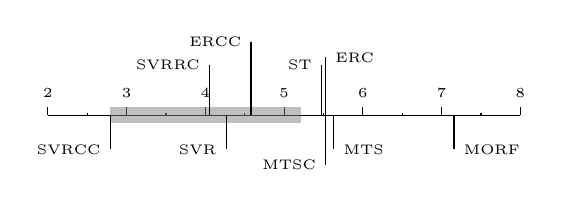
\begin{tikzpicture}
 %axis
 \draw (2,0) -- (8,0);
 \foreach \x in {2,3,4,5,6,7,8} {
  \draw (\x, 0) -- ++(0,.1) node [above] {\tiny \x};
  \ifthenelse{\x < 8}{\draw (\x+.5, 0) -- ++(0,.03);}{}
 }
 % coordinates
 \coordinate (c0) at (2.7895,0);
 \coordinate (c1) at (4.2632,0);
 \coordinate (c2) at (4.0526,0);
 \coordinate (c3) at (7.1579,0);
 \coordinate (c4) at (5.4737,0);
 \coordinate (c5) at (5.6316,0);
 \coordinate (c6) at (5.5263,0);
 \coordinate (c7) at (5.5263,0);
 \coordinate (c8) at (4.5789,0);

 % labels
 \node (l0) at (c0) [below left=.25cm and 0cm, align=right] {\tiny SVRCC};
 \node (l1) at (c1) [below left=.25cm and 0cm, align=right] {\tiny SVR};
 \node (l2) at (c2) [above left=.45cm and 0cm, align=right] {\tiny SVRRC};
 \node (l3) at (c3) [below right=.25cm and 0cm, align=left] {\tiny MORF};
 \node (l4) at (c4) [above left=.45cm and 0cm, align=right] {\tiny ST};
 \node (l5) at (c5) [below right=.25cm and 0cm, align=left] {\tiny MTS};
 \node (l6) at (c6) [below left=.45cm and 0cm, align=right] {\tiny MTSC};
 \node (l7) at (c7) [above right=.55cm and 0cm, align=left] {\tiny ERC};
 \node (l8) at (c8) [above left=.75cm and 0cm, align=right] {\tiny ERCC};

 % CD = 1.4845
 \fill[fill=gray,fill opacity=0.5] (2.7895,-0.1) rectangle (5.219,0.1);
 
 % connectors
 \foreach \x in {0,...,8} {
  \draw (l\x) -| (c\x);
 };
\end{tikzpicture}}
\caption{Bonferroni-Dunn test for aRRMSE}
\label{fig:BonfDunn}
\end{figure}

The Iman-Davenport test indicates statistically significant differences, then the Bonferroni-Dunn post-hoc test~\cite{Dunn1961} is used to find these differences that occur between the algorithms. The test assumes that the two classifiers performances are significantly different if their average ranks differ by at least some critical value~\cite{Garcia2009}. Table~\ref{tab:Bonferroni} shows the results of the Bonferroni-Dunn test on the aRRMSE rate with $\alpha = 0.05$, with the control algorithm being SVRCC. Figure~\ref{fig:BonfDunn} represents the values that are proportional to the mean rank obtained by each algorithm.  The critical difference value for our control, $2.43$, is represented in Figure~\ref{fig:BonfDunn} as the gray rectangle. The algorithms that are to the right of the critical difference rectangle and our control algorithm SVRCC, are the ones with significantly different results. Therefore, the algorithms beyond the critical difference are significantly worse. Table~\ref{tab:Bonferroni} shows the $p$-values obtained by applying the Bonferroni-Dunn procedure over the results obtained by the Friedman procedure, and it rejects those hypotheses that have an unadjusted $p$-value $\leq 6.2500E^{-3}$. From Table~\ref{tab:Bonferroni} and from Figure~\ref{fig:BonfDunn}, it can be observed that algorithms MORF, MTS, MTSC, ERC, and ST perform significantly worse. The insignificance of the results for algorithms SVR and SVRRC is due to the fact that they are algorithms with a similar base, which uses support vector regression. The same can be said for ERCC, where correlation chains have also been used, except that in SVRCC, a maximum chain is used. The results in Table~\ref{tab:Bonferroni}, obtained by the post-hoc Bonferroni-Dunn test, show that our control algorithm, SVRCC, surpasses $5$ out of $8$ algorithms. 

%Wilcoxon test (pairwise comparisons)
Table~\ref{tab:Wilcoxon} shows the results of the Wilcoxon rank-sum test~\cite{Wilcoxon1945} for aRRMSE to compute multiple pairwise comparisons among the proposed algorithms and the other competing methods. MTS performs the best among the competing methods, but SVRCC outperforms it with a confidence of approximately $92.7160\%$. Also note that the results of the Wilcoxon test show that there are significant differences between SVRCC and ERCC's performance, where SVRCC succeeds a larger number of times than ERCC.  

\begin{table}
\renewcommand{\arraystretch}{1.2}
\centering
\caption{Wilcoxon Test for aRRMSE}
\label{tab:Wilcoxon}
\begin{tabular}{cccc}
SVRCC vs. & $R^{+}$ & $R^{-}$ & $p$-value\\ 
\hline 
SVR & 175 & 15 & $5.2260E^{-4}$\\  
SVRRC & 154 & 36 & $1.5972E^{-2}$\\  
MORF & 179 & 11 & $2.0980E^{-4}$\\  
ST & 161 & 29 & $6.1800E^{-3}$\\  
MTS & 140 & 50 & $7.2840E^{-2}$\\  
MTSC & 161 & 29 & $6.1800E^{-3}$\\
ERC & 162 & 28 & $5.3300E^{-3}$\\
ERCC & 155 & 35 & $1.4070E^{-2}$\\ 
\hline 
\end{tabular}
\end{table}

This section showed the results of the experimental study with respect to the performance of our SVRCC algorithm's performance against competing multi-target methods, using the aRRMSE measure. The proposed SVRCC is generally better than the other methods, where it has the lowest average aRRMSE rate, which is statistically significant against the competing methods. We could not say that the ERCC performed worse on all counts, but looking at the aRRMSE results, we can see that it never performed the best on any of the datasets, and as the Wilcoxon test showed, it performed significantly worse. Also, considering the randomness of the chains created, along with the limited number that can be tested on, there is no guarantee that it will perform consistently with different numbers of multi-target output variables.

\section{Conclusion}\label{sec:conclusions}
The experiments performed in this study investigate the multi-target regression problem, where a model is trained using a multi-dimensional input space in order to predict a multi-dimensional output space. Despite the potential use of this type of learning, multi-target regression has been investigated less than its classification counterpart, multi-label classification. 

It has been shown that \textit{algorithm adaptation} methods perform better than \textit{problem transformation} methods due to their ability to capture relationships between target variables, which contributes positively to model training. An example of an \textit{algorithm adaptation} method would be building a regression model using ensembles of random chains of the target variables. This method however, is computationally complex, and might not capture the true correlation of the target variables.

To address this problem, this investigation introduces three novel approaches, which use a base model of Support Vector Regression and explore various techniques for solving multi-target regression problems, ensuring the correlation of the target variables is captured. Their performances are then compared to $6$ competitive \textit{algorithm adaptation} and \textit{problem transformation} methods.

The first method takes a \textit{problem transformation} approach, which generates $m$ single-target models, each trained independently of each other. This approach works well, but does not take the possible correlations between the target variables into account while training the $m$ models. This lead to our second contribution, SVRRC, which creates ensemble chained model based on $10$ random generated orders of the target variables. By using these differently ordered chains, a single ensemble model can be built based on the possible correlations of the target variables. Due to this methods computational complexity, along with the fact that the, at most $10$, randomly generated chains may not represent the targets' correlations, we proposed our final method, SVRCC. This method eliminates the computational complexity for creating chained models, and it also ensures that the relationship between the target variables is fully exploited. This relationship is captured by creating a \textit{maximum correlation chain}, where the targets are ordered in the direction of decreasing correlation. By doing this, each chained target attribute will positively contribute to the next one's prediction.  

The experiments in this paper were all conducted using the Mulan framework, MTRegressor, as well as LIBSVM's Epsilon-SVR implementation of Support Vector Regressors. Firstly, they show the superior performance of using the SVR method as a baseline model, rather than regression trees, for Multi-Target regression. They also show an increase in performance when chaining is used to develop an ensemble model, SVRRC, using random chains. This portrays the importance of the relationship among the target variables, when training a regression model. Finally, the results show the superiority of using the SVRCC method, which has the lowest average aRRMSE value for performing $10$-fold cross-validation on $19$ datasets. It performed better than the single-target SVR model and the randomly chained ensemble model SVRRC, indicating that the targets' maximum correlation contributed to SVRCC's performance. In some cases, SVR performed better, which indicates that the targets have minimal correlation to one another. The statistical analysis of these results show the statistical significance of the error rates obtained by our experiments. They showed that statistically significant differences existed between $5$ out of $9$ algorithms, where the other $4$ were our proposed methods along with the ERCC proposed by \textit{Spyromitros et. al.}. The differences were minimal for these $4$ due to their similar nature; our proposed methods all used support vector regression and the ERCC method used and ensemble of random chains. This, however, does not dismiss the findings for SVRCC. It's competitive accuracy, as well as speed (due to using a single chained model), show that it is a powerful learning algorithm for multi-target problems. 

% regular IEEE prefers the singular form
\section*{Acknowledgment}

This research was supported by the Spanish Ministry of Economy and Competitiveness, project TIN2014-55252-P, and by FEDER funds.

\bibliographystyle{model1-num-names}
\bibliography{references}

\end{document}